% !TeX encoding = UTF-8
% !TeX spellcheck = en_US


\part{Administration}
\label{part-administration}

%\section{Introduction}
%This section of the book describes which tasks and processes might need to be carried out
%on a regular basis in order to keep the application in good health and in line with
%end-users requirements.  As a result this part is more related to the functional rather
%than technical parts of the application.
%
%The fact that the tasks described in this part of the book may be recurring during the
%lifetime of the application does not exclude them from being part of the setup phase
%of LedgerSMB.  In other words: you're likely to have to dig into this section when
%creating a company as well as when maintaining it.

\chapter{Overview}
\label{cha-administration-overview}

\section{Introduction}
\label{sec-administration-introduction}

This part of the book describes the tasks and processes that may need to be carried out
on a regular basis in order to keep the application in good health and in line with
requirements from end users.

Maintenance may require different types of system access for different types of tasks:

\begin{enumerate}
\item Within application tasks, such as user management, require an appropriately authorized
   application login
\item Database administration tasks, such as creation of backups and application upgrades,
   require a database level login to be used with (amongst others) 'setup.pl'
\item Other system-level maintenance tasks, such as updating PostgreSQL or Apache, which
   require user accounts on the server hosting LedgerSMB
\end{enumerate}

Each of the above tasks requires its own type of user account. Creating and managing accounts
for the first type of task is the subject of the next chapter.

\chapter{New install}
\label{cha-new-install}

This chapter covers the general steps to use when installing LedgerSMB for the first time.
If you elected to skip Part \ref{part-getting-started} Getting Started of this document 
then this summary will
help you with the main steps normally required after installation to get LedgerSMB up and running. 

It is assumed that:
\begin{itemize}
	\item you have followed the installation instructions and have a working install.
	if not, then see the install instructions at @@@TODO.
	\item you have setup the company database using \texttt{setup.pl}.
	if not, then see the instructions at @@@TODO.
	\item  you have created an admin user with all privileges.
	if not, then see the instructions at @@@TODO.
\end{itemize} 

The basic accounting system setup steps are:

\begin{enumerate}
	\item Create a new password for the user using \menupath{Preferences \ma Password}.
	\item Setup the company defaults in \menupath{System \ma Defaults}.
	\item Edit the Chart of Accounts as necessary using \menupath{General Journal \ma Chart of Accounts}.
	This includes setting up your bank account.
	\item Enter or import customers.
	\item Enter or import vendors.
	\item Enter or import products or services.
	\item Customize Sales Order format.
	\item Customize Sales Invoice format.
	\item Customize Purchase Quotation format.
	\item Customize Purchase Order format.
	\item Testing your setup.
\end{enumerate}

\chapter{Within-application tasks}
\label{cha-within-app-tasks}

@@@TODO

\chapter{DBA tasks from setup.pl}
\label{cha-dba-tasks}

@@@TODO

\chapter{Outside-application tasks}
\label{cha-outside-app-tasks}

@@@TODO

\chapter{User management}
\label{cha-user-management}

@@@TODO

\section{Introduction}
\label{sec-user-management-introduction}

This chapter deals with management of application level user accounts. This is the first
of the three types of system access required to do LedgerSMB administration described in
the previous chapter.

\section{User creation}
\label{sec-user-creation}

Users experienced with LedgerSMB 1.2 or before or SQL Ledger (any version) are
referred to appendix \ref{sec-diff12-13-users} to read about the differences
with version 1.3.

In order to create users, the current user must be sufficiently authorized. The user
created at application set up time is such a user.

Go to the \menupath{System \ma Admin Users \ma Add User}. You'll be presented the page as shown in figure \figref{fig:create-user-step1}.

\begin{figure}[h]
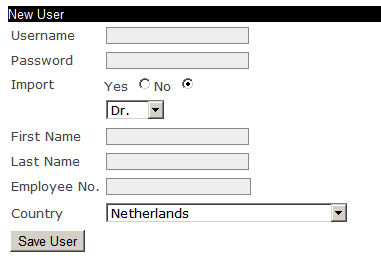
\includegraphics{create-user-step1.png}
\caption{Screen for user creation - step 1}
\end{figure}
\label{fig:create-user-step1}

The value entered in the 'Username' field will cause a database user by that name
to be created. Database users are a global resource, meaning that a collision will
occur if multiple people try to define the same user in multiple companies.
\secref{sec-user-imports} describes how to use the same user across multiple companies.

Enter the password to be used for this user into the ``Password'' field. If you're
importing a user, please leave the field empty -- that will prevent the password
from being changed.  Note that initial passwords (and password resets) are only 
valid for one day unless the user logs in and changes his/her password.

The ``Import'' field is discussed in \secref{sec-user-imports}. To create a new
user, leave the setting at ``No''.

All of the ``First Name'', ``Last Name'' and ``Employee No.'' fields are required.
However, when no employee number is specified, the system will generate one using
the sequence specified in the Defaults screen as documented in
\secref{subsubsec-company-config-defaults-item-numbers}.

The ``Country'' field speaks for itself and is required as well.


\section{User authorization}
\label{sec-user-management-authorization}

After filling out all the fields as described in the previous section and
clicking ``Save user'', you'll be presented
a second screen in the user creation process: the user authorization screen.
See \figref{fig:create-user-step2} for a screenshot of the top of that screen.

\begin{figure}[h]
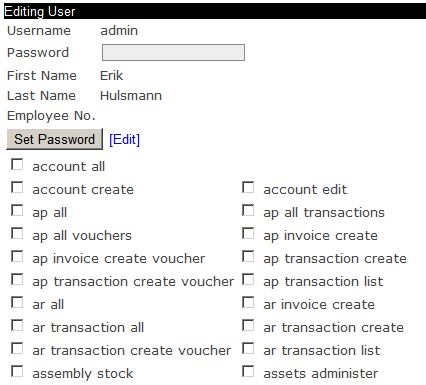
\includegraphics{create-user-step2.png}
\caption{Screen for user creation - step 2}
\label{fig:create-user-step2}
\end{figure}


The process of assigning user authorizations is the process by which the granted
access to specific parts of the application. One can imagine that - in a moderately
sized company - sales should not be editing accounting data and accountants should
not be editing sales data. Yet, in order to cooperate, both parties need to be
given access to the same application. This is where authorizations come in.

In aforementioned screen, which equals the ``Edit user'' screen, you have to assign the
newly created user his application rights. By default, the user doesn't have any
rights. Checking all check marks makes the user an application ``super user'', i.e.
gives the user all available application rights.

For a description of the roles a user can be assigned and their effects, the
reader is referred to \appref{app-role-listing}.


\section{Maintaining users}
\label{sec-user-management-maintenance}

\subsection{Editing user information and authorizations}
\label{subsec-user-maintenance-editing-authorizations}

When the role of a user in the company changes, it may be necessary to assign
that user new roles and possibly revoke some other roles. This can be done through
user search: \menupath{System \ma Admin Users \ma Search Users \ma Search \ma {[}edit]} which brings you to the same screen as presented in
\figref{fig:create-user-step2}.

Similarly, there may be reasons to change the user information, such as a last name
(e.g. upon marriage).

Note that if you reset a password, the new password is valid for one day unless
changed.  The preferred workflow is for the individual with permissions to reset
the password, give the new password to the user, they then log in and
immediately change it.

\subsection{Changing user preferences}
\label{subsec-user-management-user-prefs}

Each user can change his preferences and password through the \texttt{Preferences}
top level menu. See \figref{fig:user-preferences}.

\begin{figure}[h]
\centering
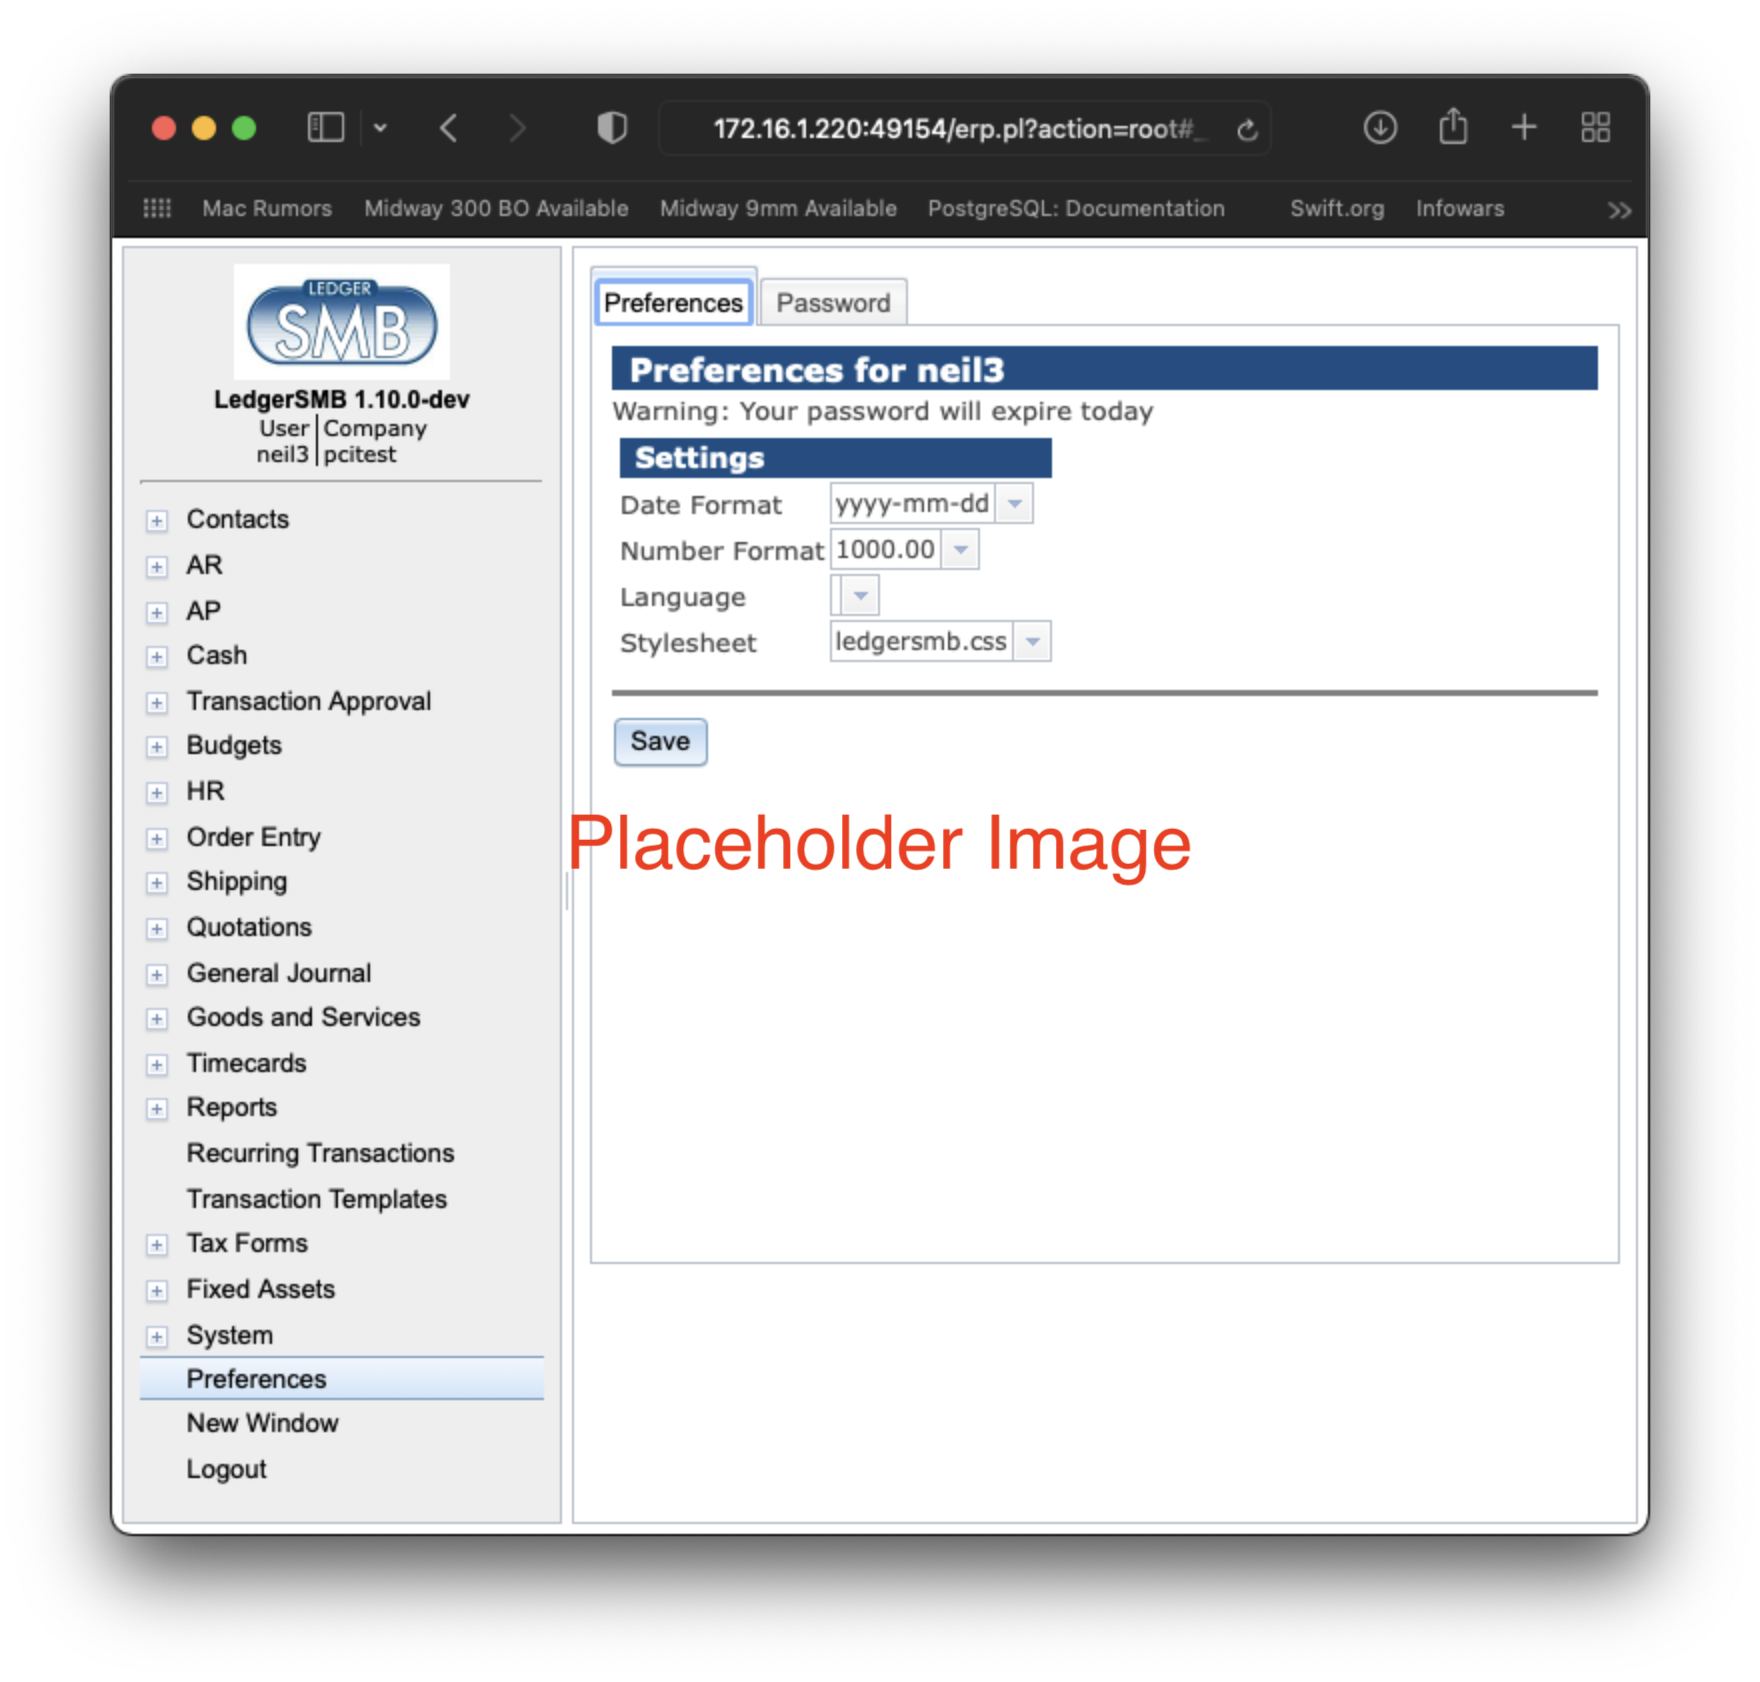
\includegraphics[width=7cm]{user-preferences.png}
\caption{User preferences screen}
\label{fig:user-preferences}
\end{figure}


\subsection{Deleting users}
\label{subsec-user-management-deletion}

From the ``User search'' result screen, users can be ``deleted'' from the company:
they have their access to the current company revoked.

\begin{quotation}
Note that the user is only revoked access to the current company; the login remains a valid
login for the database cluster. Administrators wanting to remove user accounts at the database
level need to take additional action.
\end{quotation}


\section{User imports}
\label{sec-user-imports}

If a database user already exists, e.g. because this user was created to be used
with another LedgerSMB company, it can't be created a second time. In order to be
able to use that user with the current company, it needs to be ``imported'' instead.

The difference between creating a new user and importing one is that the ``Import''
radio button should be set to ``Yes'' and that you should not fill out a password.
If you do, the password of that user will be overwritten for all companies.

All other fields are still applicable: the data entered for other companies isn't
copied to the current company.


\section{setup.pl users}
\label{sec-users-management-initial}

As mentioned in the introduction, users created through the process documented above
don't have rights to execute work with the setup.pl database administration tool.
Note that this
is on purpose. You will need access to the server to create such users, or request
one from your application service provider (ASP) if you use a hosted solution.

During the set up process such a user is normally being created. This user can later
be used to manage the database from the database administration tool setup.pl.


\chapter{Definition of goods and services}
\label{cha-products-definition}


\section{Definition of goods}
\label{sec-products-definition-goods}

Structure of products in the system.

\subsection{Definition of parts}
\label{subsec-products-parts-definition}

The part entry screen consists of four parts:

\begin{enumerate}
\item Part information
\item Vendor information
\item Customer information
\item File attachments
\end{enumerate}


The paragraphs below discuss each of the four sections. The part definition section
contains both required and optional fields. The information in the remaining
three sections is entirely optional.

\subsubsection{Part information}
\label{subsubsec-parts-information}

Every part requires the following fields to be entered:

\begin{description}[style=nextline]
\item [Number] The (alphanumeric) code the company uses to identify the item
\item [Description] The (native language) description of the item, used as the default
	description on sales invoices
\item [Inventory account] The asset account used to maintain the monetary equivalent
	of the inventory amount
\item [Income account] The P\&L (income) account to post the sales revenues on
\item [COGS account] The P\&L (expense) Cost of Goods Sold (COGS) account to use
	to post cost of sold items on
\item [Sell price] The default selling price used on sales invoices
\end{description}


The other fields in this section of the screen are optional:

\begin{description}[style=nextline]
\item [List price] Informational; can be used for any (monetary) purpose
\item [Last cost] Last buying price, updated when a vendor invoice listing the current part
    is posted
\item [Markup percentage] Markup on Last cost to calculate the Sell price
\item [Image]
\item [Drawing]
\item [Microfiche]
\item [Unit] A five-character field shown on the invoice
\item [Weight] Informational; can be used by \glspl{add-on} or customizations
\item [ROP] Reorder point - when the inventory drops below this number,
     the part will show up in ``Short parts'' reports
\item [Bin] The storage location in the warehouse
\end{description}


Apart from these fields, there are also the Make and Model paired fields. Every part
can have as many Make/Model lines as required. They are informational, but can be used
in customizations of the software.

The Average Cost and On Hand fields are output-only calculated fields. Average Cost is
calculated from the historic buying prices. On Hand is the current inventory, which is
updated when posting a vendor invoice (increased) or sales invoice (decreased).



\subsubsection{Taxation of parts}
\label{subsubsec-products-parts-taxation}

Right below the accounts selection section, there is the Tax section, which lists
all tax accounts with a check mark. Each account corresponds with a certain tax type
and rate. E.g. in the Netherlands, there's one VAT tax type (BTW) which has two rates,
one of which applies to every product. This setup requires two accounts. There's more
on the subject of sales taxes in \charef{cha-taxes}.

By checking the checkmark on an account, the system is signalled to calculate that
kind of tax for the part {\it if the customer (or vendor) has the appropriate setup}
as described in section


\subsubsection{Vendor information}
\label{subsubsec-parts-vendor-information}

This section of the screen lists one or more vendors from which the part can be
purchased, with purchasing information for the given vendor:

\begin{description}[style=nextline]
\item [Vendor code] Code used by the vendor to identify the good, to be used by
    customizations and future enhancements (currently informational only)
\item [Lead time] Lead time of the part from the vendor in days
\item [Last cost] Last price at which the good was purchased from the vendor
\item [Currency] The currency belonging to the Last cost field
\end{description}

\subsubsection{Customer information}
\label{subsubsec-parts-customer-information}

The customer information section specifies sell prices per customer or price group
where those are required to deviate from the default sell price. This mechanism exists
to support the marketing principle of categorizing customers.

\begin{description}[style=nextline]
\item [Sell price] Price for this part to be used for this customer
\item [From] Start of the applicability window of the price (inclusive)
\item [To] End of the applicability window of the price (inclusive)
\end{description}

\subsubsection{File attachments}
\label{subsubsec-parts-file-attachments}

The process of attaching files to parts is very similar to that of
attaching files to quotations, which is covered in \secref{sec-workflows-quotations-file-attachments}.

\subsection{Definition of part groups}
\label{subsec-parts-groups}

All goods and services can be categorized in 'part groups'. Upon lookup, these can
help to limit the number of matches when searching for a partial part number.

As long as no part groups have been defined, the part group assignment field doesn't
show up on the goods entry screens.

There's no requirement that a good be assigned to any specific part group if part
groups have been configured, however, a good can be assigned to more than one part group.

\subsection{Definition of assemblies}
\label{subsec-assemblies-definition}


\subsection{Definition of overhead or labor}
\label{subsec-overhead-definition}

\subsection{The use of parts versus assemblies for multi-item-package sales}
\label{subsec-parts-versus-assemblies}

Often times, one may want to sell pre-packaged multiples of a single item, such as Jack
in \charef{cha-building-up-stock} who wants to sell memory modules in pairs as well as
single items, with the price for the pair set separately from the single-item price.

There are basically two use-cases

\begin{enumerate}
\item Pre-packaged sales which are separately stocked
\item Single item sales which are achieved by unwrapping the multi-item packages
\end{enumerate}

The former case would be that of a supermarket selling packages of coffee in
singles and shrink-wrapped in pairs. These items get stocked, sold and produced separately.
Handling these is straight forward: as they are basically separate products from the point
of administration and inventory management, they're handled as separate parts.

The latter case would be Jack's case where single-item sales is achieved by unwrapping
a multi-item package. Basically, there's a single inventory for both types of packaging.
This situation can be handled (a) by creating separate parts or (b) by creating a part and an
assembly.
To reiterate: The fact that one wants to be able to separately set a pricing strategy
for the bundled items is the driver to go look for other solutions than just sell a
multiple of the original item.

There is no option which matches the actual practice: one inventory for two parts. The solution
always will keeps two separate stocks for the two items, but one may work better in practice
than the other.

Option a (separate parts) keeps the inventory of both items strictly separate,
meaning there's no way to convert between the two, other than selling and buying.

Option b (a part and an assembly) mismatches reality in so far that it will require one
to stock the single items and update the assembly stock regularly while in practice the
multi-item packages are stocked and unwrapped upon single-item sales. This procedure works
to have the assembly stock go negative on sales and restock regularly (e.g. daily) to
update assembly stock back to 0 (zero). This removes inventory from the single-item stock,
allowing for a semi-automated way to convert stock from one type of inventory to another.


\section{Definition of services}
\label{sec-products-services-definition}

\subsection{Taxation of services}
\label{subsec-products-services-taxation}



\chapter{Chart of accounts}
\label{cha-chart-of-accounts}

\section{Accounts and headers}
\label{sec-coa-accounts-and-headers}

The system allows ordering accounts into groups by assigning accounts to headers. Headers
can themselves be assigned to other headers resulting in trees of account groups.\footnote{Although the
	 database structure supports this type of account hierarchy from  1.3, it was not fully in use in reports until  1.4.17. In 1.3 accounts can be assigned a header,
but headers can't be assigned to headers themselves.}



\section{Account configuration}
\label{sec-coa-account-configuration}

Headers don't have any configuration, other than their number and description. Accounts also
have a number and description, but require additional configuration for the application to work
correctly. The settings are described in the sections that follow.

\subsection{Account options}
\label{sec-coa-account-options}
\begin{description}[style=nextline]
\item[Contra] This checkmark identifies the account as a \gls{contra} account, which means
   that the account is going to hold the opposite of an account it's associated with.
   A good example of this kind would be the depreciation account associated with a fixed
   asset account where the depreciation account contains the credit amount to be added to
   the original asset (debit) value to get the current asset value.
\item[Recon] This checkmark identifies the account as one which needs reconciliation as
   described in \secref{sec-workflows-accounting-reconciliation}.
\item[Tax] This checkmark identifies the account as a Tax (VAT) account. Tax accounts need
   to be further configured. See \charef{cha-taxes} for further discussion of the
   subject.
   \label{item:AccountOptionsTax}
\end{description}

\subsection{Summary accounts}
\label{subsec-coa-summary-accounts}

There are currently three types of summary accounts:

\begin{enumerate}
\item AR Marking an account as a summary account for AR means that all outstanding
   receivable amounts will be posted to this account. The Accounts Receivable administration
   will contain the details of which amount is owed by which customer.
\item AP Same as the AR account, except for amounts owed to vendors.
\item Inventory This account holds the monetary value equal to the items on stock.
\end{enumerate}

\subsection{Account inclusion in drop down lists}
\label{subsec-coa-account-links}
@@@ Add summary

\subsubsection{Receivables \& payables UI}
\label{subsubsec-coa-AR-AP-checkmarks}

\begin{description}[style=nextline]
\item[Income (AR\_amount)] This check mark adds the account to the list of accounts
   in the transaction and invoice screens which are used to post income on.
\item[Payment (AR\_paid)] This check mark adds the account to the list of accounts
   to choose from in the Receipts (AR) and Payments (AP) screens. Additionally, it
   adds the account to the part entry screen as described in \secref{subsec-products-parts-definition}.
\item[Tax (AR\_tax)] This check mark makes the account show up as a check mark on the
   customer (AR) or vendor (AP) entry screen. See \charef{cha-taxes} for further discussion.
\item[Overpayment (AR\_overpayment)] Adds the account to the receipts screen as discussed
   in \secref{sec-workflows-payment-processing-overpayments}.
\item[Discount (AR\_discount)] Adds the account to the customer entry screen's selection
   list for accounts to post 
\end{description}

The payables UI works the same way as the receivables UI. The difference is
that the technical names of the configuration identifiers are prefixed by AP\_ instead
of AR\_.

\subsubsection{Tracking Items}
\label{subsubsec-coa-tracking-items}

The items on this line relate to stocked items, i.e. those tracked for inventory: parts and
assemblies.

\begin{description}[style=nextline]
\item[Income (IC\_sale)] Adds the account to the selection list of income accounts on the
   part and assembly definition screens.
\item[COGS (IC\_cogs)] Adds the account to the selection list of COGS @@@ accounts on the
   part, assembly and overhead definition screen.
\item[Tax (IC\_taxpart)] Adds a check mark to the part and assembly definition screen
   for the applicable account. See \charef{cha-taxes} for more details on how taxes
   work in LedgerSMB.
\end{description}

@@@ Question: Labor/Overhead accounts == inventory accounts??
  % Labor/Overhead has an inventory and expense account but no income account.
  % Chris T

\subsubsection{Non-tracking items}
\label{subsubsec-coa-non-tracking-items}

The items on this line relate to untracked (non stocked) items, i.e. services.

\begin{description}[style=nextline]
\item[Income (IC\_income)] Adds the account to the income account selection list in
   the service definition screen.
\item[Expense (IC\_expense)] Adds the account to the expense account selection list in
   the service definition screen.
\item[Tax (IC\_taxservice)] Adds a check mark to the service definition screen for the
   applicable account. See \charef{cha-taxes} for more details on how taxes work in LedgerSMB.
\end{description}

\subsubsection{Fixed assets}
\label{subsubsec-coa-fixed-assets}

\begin{description}[style=nextline]
\item[Fixed asset (Fixed\_Asset)] Marks the account as holding the original asset value for the fixed
   assets module, for some classes of fixed assets.
\item[Depreciation (Asset\_Dep)] Marks the account as holding the cumulative depreciation amount
   for the fixed assets module, for some classes of fixed assets.
\item[Expense (asset\_expense)] Adds the expense account to the selection list of the fixed assets
   accounting module. See \secref{sec-workflows-accounting-fixed-asset-accounting} for more details.
\item[Gain (asset\_gain)] Account to hold book value gain upon disposal of a fixed asset.
\item[Loss (asset\_loss)] Account to hold book value loss upon disposal of a fixed asset.
\end{description}

\subsubsection{Importing chart of accounts}
\label{subsubsec-coa-importing}

\section{Alternative accounts (GIFI)}
\label{sec-coa-gifi}

Next to the regular account numbering scheme, LedgerSMB supports a second
numbering scheme: GIFI numbering. \gls{gifi} is a standardized account 
coding system used in Canada by the Canada Revenue Agency for processing
corporate Tax Returns forms. 

Other countries (e.g. France) may have required numbering schemes for
corporate accounting as well.

If you use GIFI account numbers, each account is associated with a GIFI
account. Multiple accounts may map to a single GIFI account.

Many General Ledger reports exist in two variants: a variant using the
normal G/L accounts and one with the GIFI numbering scheme. In the GIFI
variant, when a single GIFI has multiple accounts, the total reported
under GIFI is the sum of the mapped accounts.


\subsection{Maintaining GIFI}
\label{subsec-coa-gifi-maintenance}

GIFI accounts should be created before being assigned to a standard G/L account. GIFI accounts
can be maintained through the \menupath{System \ma Chart of accounts \ma Add GIFI} and List GIFI menu items. Existing accounts can be edited by selecting them from the List GIFI menu, which opens a page where individual GIFI items can have their number or
description adjusted.


\chapter{Taxes}
\label{cha-taxes}

\section{Overview}
\label{sec-tax-overview}

When an account has been marked as a Tax account (see \secref{sec-coa-account-options}, item
\ref{item:AccountOptionsTax}) several things happen:

\begin{itemize}
\item The account will be shown in the customer and vendor account screens with
   a check mark to mark it ``relevant for the customer''
\item The account will be shown in the part and service configuration screens
   with a check mark to mark it ``relevant for the part/service item''
\item The account will be shown in the tax configuration screen in order to set
   a tax percentage on the account as discussed in the next section
\end{itemize}

By marking an account relevant for a customer, taxes will be calculated when
creating a sales invoice for the given customer which includes parts which also
have the specific account marked as relevant.

\section{Tax account configuration}
\label{sec-tax-account-configuration}

\begin{figure}[h]
\centering
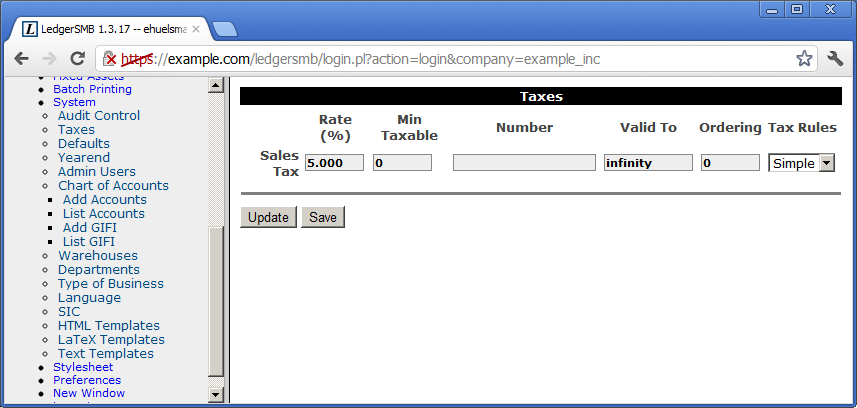
\includegraphics[width=7cm]{setup-tax-rates.png}
\caption{Tax account configuration screen}
\end{figure}
\label{fig:tax-account-config-screen}

The screen (shown in \figref{fig:tax-account-config-screen}) presents a table with
the full history of the percentage rates, their dates of applicability and the tax
accounts they apply to. An account can show up any number of times, with different
Valid To dates.

\begin{description}[style=nextline]
\item [Account name] The first column; not an input field
\item [Rate (\%)] The rate to be applied to the sales amount
\item [Min Taxable] The minimum amount for which the tax is applicable
\item [Number] The tax reporting number to be used for this tax
\item [Valid To] Date until which the tax rate is applicable
\item [Ordering] The meaning of this field is described below
\item [Tax Rules] The selection list presents a list of available 'tax rules engines'. By
   default the list consists of the 'Simple' module only, which is the engine which comes
   with LedgerSMB; the reader is referred to \secref{sec-tax-rule-plugins} for a more detailed
   description of this subject
\end{description}

To determine which line is applicable at any time, order the lines by their validity date and
select the first one for which the validity date is later than the date being checked for. E.g.
if you have two lines - one with a Valid To date of 2010-01-01 and one with a Valid To date of
``infinity'' - the 2010 line would be selected when checking for a date in 2009 while the ``infinity''
line would be selected for any date later than Jan 1st, 2010. This facilitates advance entry of a new
tax rate in case of a rate change if a tax rate changes: the new rate will automatically be selected
beyond the validity date of the old rate.

The order field is used to layer taxes, e.g. Canada where the province of Quebec taxes
the taxes collected by the national authority, which works like this numerically:
National tax with order 0 and rate 10\% and Quebec tax with order 1 and rate 5\%
applied to a 10\$ amount charges 1\$ of national tax and 0.55\$ of Quebec tax (5\% of 11\$).

\begin{quotation}
Note that - as pointed out in the Overview section of this chapter - the customer related
tax calculation on invoices is triggered by the settings in this chapter as well as
the customer/vendor settings described in \secref{sec-workflows-creating-customers-and-vendors}
and part settings and service settings described in \secref{subsubsec-products-parts-taxation} and
\secref{subsec-products-services-taxation} respectively.
\end{quotation}

\section{Tax calculation examples}
\label{sec-tax-calculation-examples}

% ### TODO

\section{Tax calculation plug-ins}
\label{sec-tax-rule-plugins}

The tax calculation system has been designed to handle the most complex tax system
thinkable. Because the tax calculation rules for most set ups aren't really all that
complex, LedgerSMB comes with a single tax calculation plug in out of the box: the
``Simple'' tax calculation rule.

For more complex needs, more complex routines can be developed and plugged into
LedgerSMB side-by-side with the simple rule.


\section{Tax forms}
\label{sec-tax-taxforms}

The tax forms facility exists to help file sales tax forms. It's primarily modelled
after the 1099 US tax reporting forms functionality, which means that it's cash based.
The fact that it's cash based means that invoices will be included in the tax report
as soon as cash for the invoice is received. Accrual based reporting means that the
tax is reported based on the invoice date instead of the payment date.

This system can only be used in some EU countries and by some companies at that: the
country needs to allow cash based reporting and the company needs to have filed
for cash based reporting as well.

Before using this functionality be sure to check with an accountant or the tax
authorities if cash based reporting is appropriate.

\subsection{Overview}
\label{subsec-tax-taxforms-overview}

Tax forms are meant to support tax reporting requirements in the countries
where the company has tax reporting obligations. This means that tax forms
are country specific: each country for which reporting obligations exist
needs to have its own form associated.

In order to be able to collect taxes in a tax form companies need to be
linked to it. \secref{subsec-workflows-customers-creating-account} describes how to do this.

When associations have been set up between companies and
tax forms, the ``Tax form'' check mark can be used in invoices to include
(or exclude) invoice lines from the tax form. See \secref{subsec-workflows-invoicing-manual-entry-invoices}
for entry of invoices.

\begin{quotation}
Note that there's a module available for 1.3 which implements accrual based tax reporting by
the name of EU VAT reporting. This module replaces the default tax reporting functionality
meaning one can only have accrual based or cash based reports in a single company at this time,
but not both.
\end{quotation}

\subsection{Creating tax forms}
\label{subsec-tax-taxforms-creation}

Tax forms can be created (or edited) using the menu options available under the
``Taxforms'' main menu item.

Tax forms have three fields.

\begin{description}[style=nextline]
\item [Country] Country to which the tax form applies
\item [Description] Name of the tax form to be displayed in drop down lists
\item [Select by Default] % ### TODO verify: Determines if the tax form check mark on invoices is checked  or unchecked by default
\end{description}



\chapter{Pricing}
\label{cha-pricing}

\section{Introduction}
\label{sec-pricing-introduction}

In the application there are four reasons for an invoice to include a discount:

\begin{enumerate}
\item Because a discount is entered by the sales person creating the quotation,
  sales order or sales invoice
\item Because the customer's payment terms include a discount for paying early
\item Because the customer belongs to a type of business which is entitled to discounts
\label{item:PricingBusinessType}
\item Because the customer has been assigned a price matrix leading to discounts
\label{item:PricingPriceMatrix}
\end{enumerate}

This section deals with items \ref{item:PricingBusinessType} and \ref{item:PricingPriceMatrix} only.

@@@ types of business are 'old school'; price groups have been introduced to replace types of business with a more fine-grained structure.

\section{Definition of types of business}
\label{sec-pricing-business-types}

Types of business are really straight forward: they feature a description
which allows them to be identified in the customer account screen and a discount
percentage which is applied across the board. I.e. all invoices to the customer
will have that discount applied.

\section{Definition of price groups / price matrix}
\label{sec-pricing-price-groups}

\chapter{Contingency planning}
\label{cha-contingency}

\section{Backup and restore}
\label{sec-contingency-backup-restore}

\subsection{Backup using setup.pl}
\label{subsec-contingency-backup-setup-pl}


\subsection{Backup using PostgreSQL administration tools}
\label{subsec-contingency-backup-psql}

\subsection{Restore}
\label{subsec-contingency-restore}

\begin{quotation}
Note that if the database being restored is a backup from a different (earlier) PostgreSQL version,
additional steps described in \appref{sec-migration-postrgesql} will be required.
\end{quotation}




\section{Advanced PostgreSQL: replication}
\label{sec-contingency-replication}


\chapter{Software updates}
\label{cha-software-updates}

\section{Introduction}
\label{sec-updates-introduction}

This chapter describes patch release updates. Upgrades from older versions (e.g. 1.1 or 1.2)
are covered in \appref{app-migration}. The same is true for upgrades from SQL Ledger 2.6 or 2.8.

The remainder of the chapter discusses the steps to be executed. Please note that the instructions
below mean a window where the application can't be used during the entire execution of the procedure.

\section{Backups}
\label{sec-updates-backups}

\begin{itemize}
\item Backup database roles (authorizations)
\item Backup database content (structure and data)
\item Backup software and settings files
\end{itemize}



\section{Software upgrade}
\label{sec-updates-software-upgrades}

@@@ Untar / use package manager

\section{Database upgrade}
\label{sec-updates-database-upgrades}

@@@ go to setup.pl and ``Rebuild''

\chapter{Optional Features}
\label{cha-options}

As business requirements change sometimes it may be necessary to add or remove
some of the optional features of LedgerSMB.  This chapter describes how these
optional features work, how to troubleshoot them of things go wrong, and how to
enable or disable them.

\section{PDF and Postscript Documents}
\label{sec-options-pdf}

LedgerSMB can create PDF and Postscript documents for orders, invoices, and
more.  This is an optional feature and requires some additional software not
included with LedgerSMB, including a \LaTeX\ distribution and extensions to 
Perl's TemplateToolkit framework.

The PDF and PS invoices are generated using a program called \LaTeX\
which handles the layout and typesetting.  The actual \LaTeX\ files are
creating using Template Toolkit with extensions for \LaTeX.  These
extensions are in the Template::Latex package available from CPAN.
The software then generates a \LaTeX\ file which is then processed to
create a PDF or PS.

Typically the first thing to do is to install a \LaTeX\ distribution
like TexLive (distributed with many Linux distributions and available
for OSX and Windows).  This provides \LaTeX\ and many of the modules
needed.   In general I recommend that if your distro has a
texlive-extras package that you install this too.

After this is installed, you must then install Template::Latex.  This
can be done by typing on the command line:

\# cpan Template::Latex

This will also install a number of dependencies including
LaTeX::Driver, which will need to know where your LaTeX binaries are.
It is usually pretty good at finding them.

If things go wrong and you can't get it to work, the following
commands may provide useful diagnostic information when requesting
help:

From the LedgerSMB application directory:
\$ perl -MLedgerSMB::Template::Latex -e print

From the doc/manual directory in the LedgerSMB application directory:
\# pdflatex LedgerSMB-manual

\section{Attaching Uploaded Files to PDF Invoices}
\label{sec-options-uploaded-files-invoices}

\section{OpenDocument Spreadsheet Output}
\label{sec-options-ODS-spreadsheet-output}


\section{Microsoft Excel Output}
\label{sec-options-XLS-spreadsheet-output}

